\documentclass[11pt,letterpaper]{article}
%\documentclass[11pt,a4paper]{report}

\usepackage{amssymb,amsmath,amsthm} 
\usepackage[margin=2cm]{geometry}
\usepackage{fancyhdr}
\usepackage{enumitem}
\usepackage[compact]{titlesec}
\usepackage{graphicx,ctable,booktabs,subcaption}

\usepackage{xparse,hyperref,parskip}

%\newcommand{\abs}[1]{\left|#1\right|}

\newcommand{\semester}{Spring 2022}
\newcommand{\due}{Tuesday, March 1}


\pagestyle{fancy}
\lhead{ }
\chead{\footnotesize Math 3338\quad  Numerical Methods\quad  \semester}
\rhead{\footnotesize \thepage}
\setlength{\parindent}{0cm}
\setlist{noitemsep}



\newtheorem{theorem}{Theorem}

\input{defs.tex}

%Defines the problem environment with arguments Points and Solution gap
\input{problem_env.tex}



\begin{document}

\begin{center}
{\huge{\bf  Numerical Methods}} \\[1.5ex]
{\bf Math 3338 -- \semester}\\[1.5ex]
{\Large{\bf Worksheet 13\ \\[2ex] Solutions to Non-Linear Equations}}\\
\end{center}
\vspace{2mm}


\section{Reading}

\begin{table}[!ht]
 \centering
 \begin{tabular}{ll}
   CP &  6.3 \\
 NMEP &  Chapter 4
 \end{tabular}
\caption{Sections Covered}
\end{table}

\section{Solving}

Solve the following,
\[
2x+3 = 0
\]
Now solve this,
\[
x^2-3x-4 = 0
\]
How about,
\[
x^5-4x^3+2x-1 = 0
\]
Finally,
\[
e^x = x+3
\]

The question you should be asking is \emph{do these actually have solutions?} and \emph{how many 
solutions are there?}. The first two are easy. We know the third
one has at least one real root, it's an odd degree polynomial. The fourth one probably has two
roots, based on what we know about $e^x$. The real way to tell is to draw a graph. Figure \ref{fig:exa}
shows both of these functions.

\begin{figure}[!ht]
 \centering
 \begin{subfigure}{.4\textwidth}
  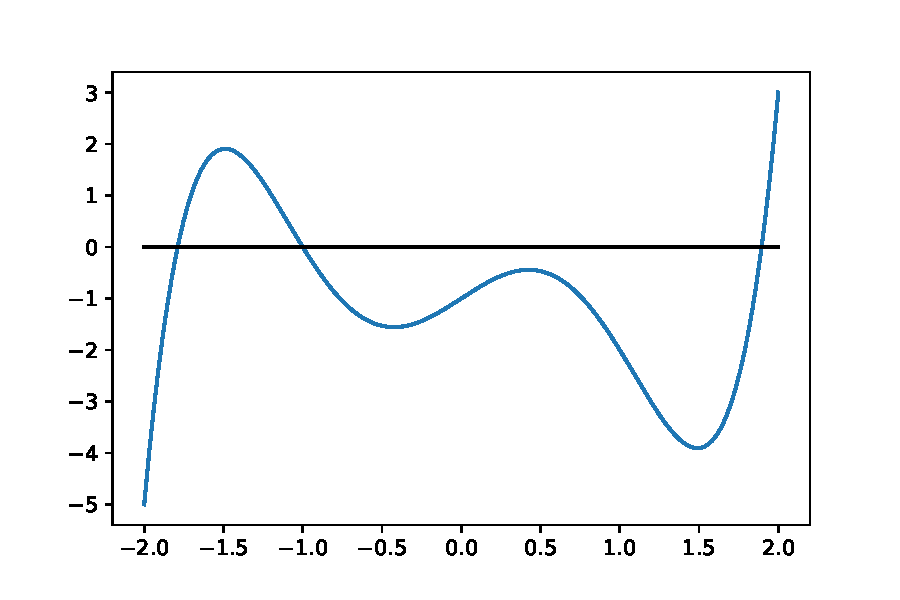
\includegraphics[width=.8\textwidth]{images/exa1.pdf}
 \end{subfigure}
 \begin{subfigure}{.4\textwidth}
  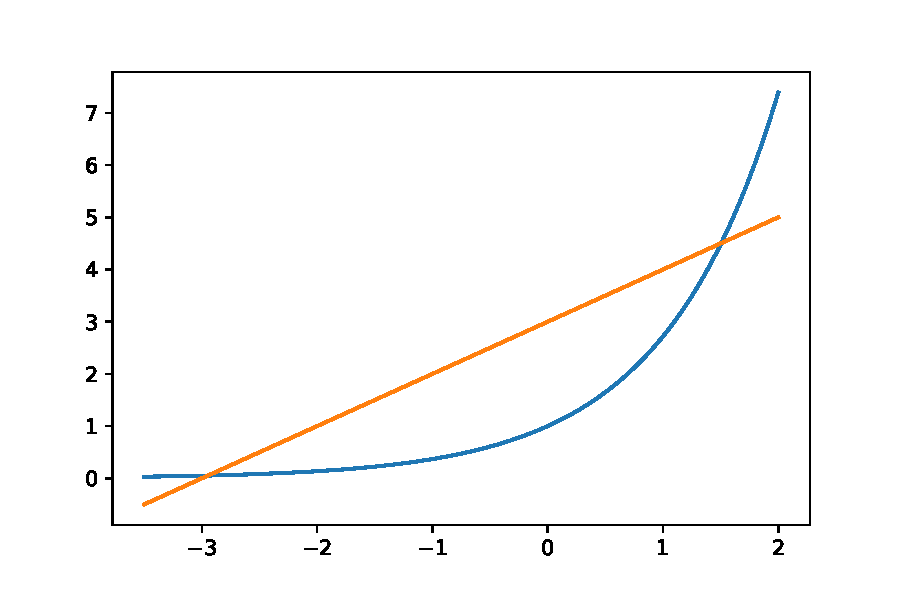
\includegraphics[width=.8\textwidth]{images/exa2.pdf}
 \end{subfigure}
 \caption{The graphs. Figure out which is which.}
 \label{fig:exa}
\end{figure}

The graphs don't actually tell use the solutions. It may look like $x=-3$ is a solution to
$e^x=x+3$, but it clearly isn't.

\section{The Bisection Method}

Suppose $f(a)<0$ and $f(b)>0$. We can get closer to the zero by
evaluating $x = \frac{b-a}{2}$ and computing $f(x)$. If $f(x)>0$ then the zero is in 
the range $[a,x]$, if $f(x)<0$ then it's in $[x,b]$ if $f(x)=0$, then you should probably
stop.

Since this method halves the width of the interval at each iteration, it will converge quite
quickly.

\section{Newton's Method}

This is a much, much faster way to approximate the zero of a polynomial. The basic idea to
approximate the curve by a line (tangent line) and solve that line. The tangent line should approximate
the curve, so the zero should be close to the actual zero. The closer you start to the zero, the 
closer the approximation should be. You then iterate.

In general, Newton's method follows the recursion,
\[
 x_{n+1} = x_n - \frac{f(x_n)}{f'(x_n)}
\]
where $x_0$ is a point ``close'' to the zero.

You may have noticed a liberal use of the word ``should''. There is are several reasons for that,
first we are dividing by $f'(x)$, what if this is zero? Second, if we choose a bad initial point,
the tangent line could go far away from the zero. We won't concern ourselves with these issues...
At least not today.

\newpage

\begin{center}
{\huge{\bf  Numerical Methods}} \\[1.5ex]
{\bf Math 3338 -- \semester}\\[1.5ex]
{\Large{\bf Homework 12 (Due: \due)}}\\
\end{center}
\vspace{2mm}

\begin{problem}
 Write a program to compute a zero using the bisection method. Call this function
\texttt{bisection(f,a,b,tol = 1e-6)} where $f$ is the function, you are searching $a\le x\le b$
and $tol$ is the tolerance you desire.
\end{problem}

\begin{problem}
 Write a function to compute a zero using Newton's method. Call this function 
\texttt{newton(f,fp,a,tol=1e-6)} where $f$ is the function, $fp$ is the derivative, $a$ is the
starting point and $tol$ is the tolerance you desire.
\end{problem}


\begin{problem}
 Write a function to compute a zero using Newton's method, except this time we will numerically 
calculate the derivative. Call this function \texttt{newton\_numeric(f,a,tol=1e-6)} where $f$ is the 
function, $a$ is the starting point and $tol$ is the tolerance you desire. Compute the derivative
numerically, you could be clever here and use the points $x$ and $x'$ from successive steps
of Newton's method (it's not required to do it this way).
\end{problem}



\begin{problem}
 Compare computation times for each of your functions. Do do this, use the given table of functions
with given inputs. Calculate to an accuracy of $1e-12$. Since these calculations will be very fast,
run each one 10000 times and find the total time. In other words, start the timer, run 10000 times,
and stop the timer. The total computation should take less than 1 minute (it took approximately 
10 seconds on my laptop).

\begin{table}[!ht]
\centering
 \begin{tabular}{cccc}
 Function & $x_0$ & $a$ & $b$ \\ \hline
 &  & &  \\[-2ex]
$x^5-4x^3+2x-1$ & $-2$ & $-2$ & $-1.5$ \\
$x^5-4x^3+2x-1$ & $-1$ & $-1.5$ & $1$ \\
$x^5-4x^3+2x-1$ & $2.5$ & $1.5$ & $3$ \\
$e^x=x+3$ & $-3$ & $-4$ & $-2$ \\
$e^x=x+3$ & $2$ & $1$ & $2$ \\
 \end{tabular}
\end{table}
\end{problem}




\end{document}



































